\newpage
\changeindent{0cm}
\section{提案手法}
\changeindent{2cm}

本章では, Knowledge Graph 補完および, 本研究における提案手法についての説明をする. 本研究における提案手法はモデルの提案とモデルの学習方法の提案に分けられる. これらの提案手法により, 言語情報を含む Knowledge Graph を扱う従来研究の問題点の解決を目指す. \par
Knowledge Graph 補完について説明する. Knowledge Graph のある Triple における Head, Relation, Tail をそれぞれ h, r, t とすると, Knowledge Graph 補完では Triple (h, r, t) に対して ``t" に入る Tail を回答することで Entity 間の関係性を予測する. \par
従来の Knowledge Graph 補完手法として Knowledge Graph Embedding 手法である TransE \cite{TransE_WN18} や ComplEx \cite{ComplEx} などがある. これらの手法は Entity と Relation をそれぞれ実数値ベクトルとして表し, それらのベクトルの関係式を用いて Triple の妥当性を評価する. \par
例えば TransE では, まず Entity と Relation をそれぞれ $d$ 次元の埋め込み表現にする. このとき, 与えられる埋め込み表現はランダムに初期化されたベクトルとする. 次に Triple を構成する Head, Relation, Tail の埋め込み表現 $\bm{v}_{\rm h}$, $\bm{v}_{\rm r}$, $\bm{v}_{\rm t}$ に対して, すべての Triple が ``$\bm{v}_{\rm h} + \bm{v}_{\rm r} = \bm{v}_{\rm t}$" を満たすように埋め込み表現を学習する. これにより Head と Relation から Tail を予測することができる. \par
このように, 既存の Knowledge Graph 補完手法は Triple の構造情報を重視した手法となっており, Entity 自体の意味情報を重視して補完する形ではないという特徴が挙げられる. \par
本研究では, Entity 自体の意味情報を効果的に捉えるために BERT を MLM で fine-tuning したモデルを用いて, 1 つのシーケンス (Head, Relation, [MASK]) を入力文として Tail を予測することによる Knowledge Graph 補完手法を提案する. 図 \ref{KG-MLM} に提案手法のモデル概略図を示す. 図 \ref{KG-MLM} の Tok はトークンを, $\bm{E}$, $\bm{T}$ は埋め込みベクトルとモデルの出力のベクトルをそれぞれ示す. $l, m, n$ は Head, Relation, Tail のトークン数を, h, r, t は Head, Relation, Tail をそれぞれ表す. 入力シーケンスの最初のトークンは常に特別なトークン ``[CLS]" である. Head はトークン ${\rm Tok}_{1}^{\rm h}, …,{\rm Tok}_{l}^{\rm h}$ を含む文, Relation はトークン ${\rm Tok}_{1}^{\rm r}, …,{\rm Tok}_{m}^{\rm r}$ を含む文, Tail はトークン ${\rm Tok}_{1}^{\rm t}, …,{\rm Tok}_{n}^{\rm t}$ を含む文で表現される. Head, Relation, Tail の文は特別なトークン ``[SEP]" で区切られる. このトークン列のうち, Tail の見出し語のみ, もしくは Tail 全体を ``[MASK]" トークンに置き換えたシーケンスを BERT への入力とする. これにより, ``[MASK]" トークンとした箇所の予測単語が出力される. \par

\begin{figure}[t]
    \centering
    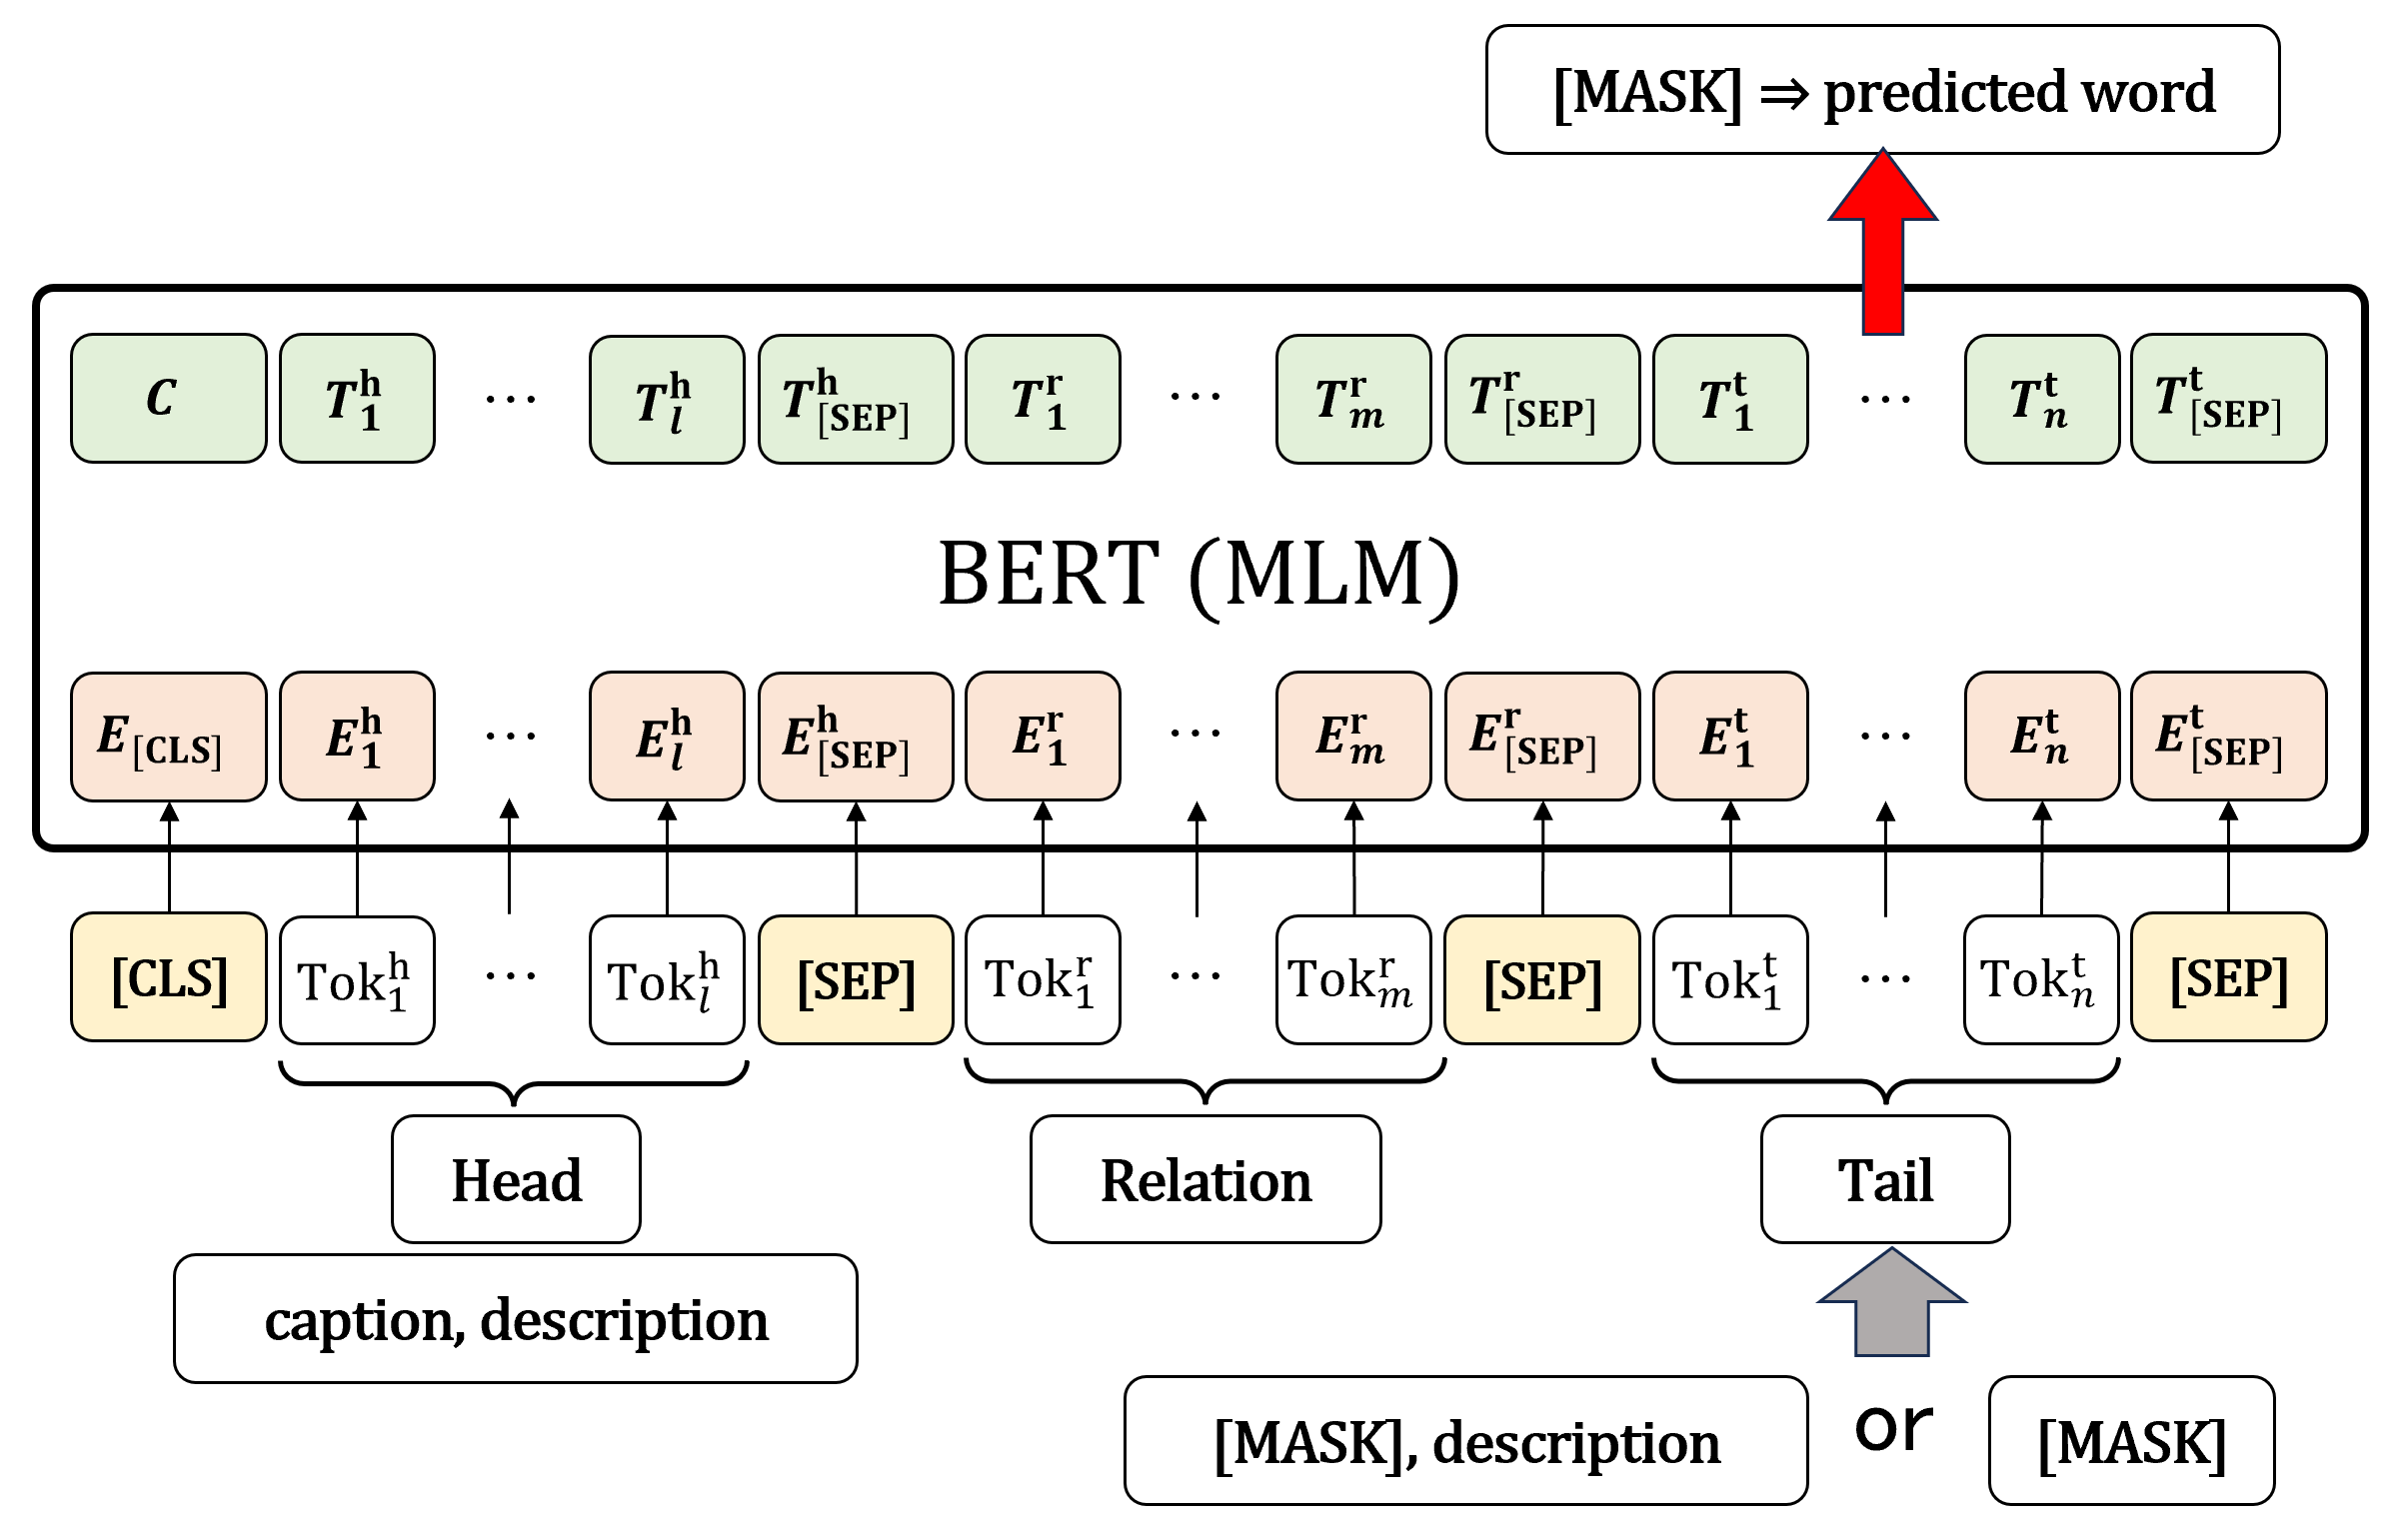
\includegraphics[width=16cm]{assets/KG-MLM.png}
    \caption{提案手法のモデル概略図}
    \label{KG-MLM}
\end{figure}

図 \ref{MLM_fine_tuning} に BERT の MLM による fine-tuning の概略図を示す. 図 \ref{MLM_fine_tuning} の記号は図 \ref{KG-MLM} の記号と同様である. 入力シーケンスの最初のトークンは常に特別なトークン ``[CLS]" である. Head はトークン ${\rm Tok}_{1}^{\rm h}, …,{\rm Tok}_{l}^{\rm h}$ を含む文, Relation はトークン ${\rm Tok}_{1}^{\rm r}, …,{\rm Tok}_{m}^{\rm r}$ を含む文, Tail はトークン ${\rm Tok}_{1}^{\rm t}, …,{\rm Tok}_{n}^{\rm t}$ を含む文で表現される. Head, Relation, Tail の文は特別なトークン ``[SEP]" で区切られる. さらに, BERT が提案された論文 \cite{BERT} と同様に入力トークンの 15\% のうち, 80\% を ``[MASK]" トークンに置き換え, 10\% をランダムなトークンに置き換え, 10\% をそのままのトークンにする. そして, 入力トークンの 15\% に Tail の見出し語を必ず含むように設定する. このシーケンスを BERT への入力とし, ``[MASK]" トークンとした箇所, もしくはランダムなトークンとした箇所の予測単語が元の単語となるように学習する. \par

\begin{figure}[t]
    \centering
    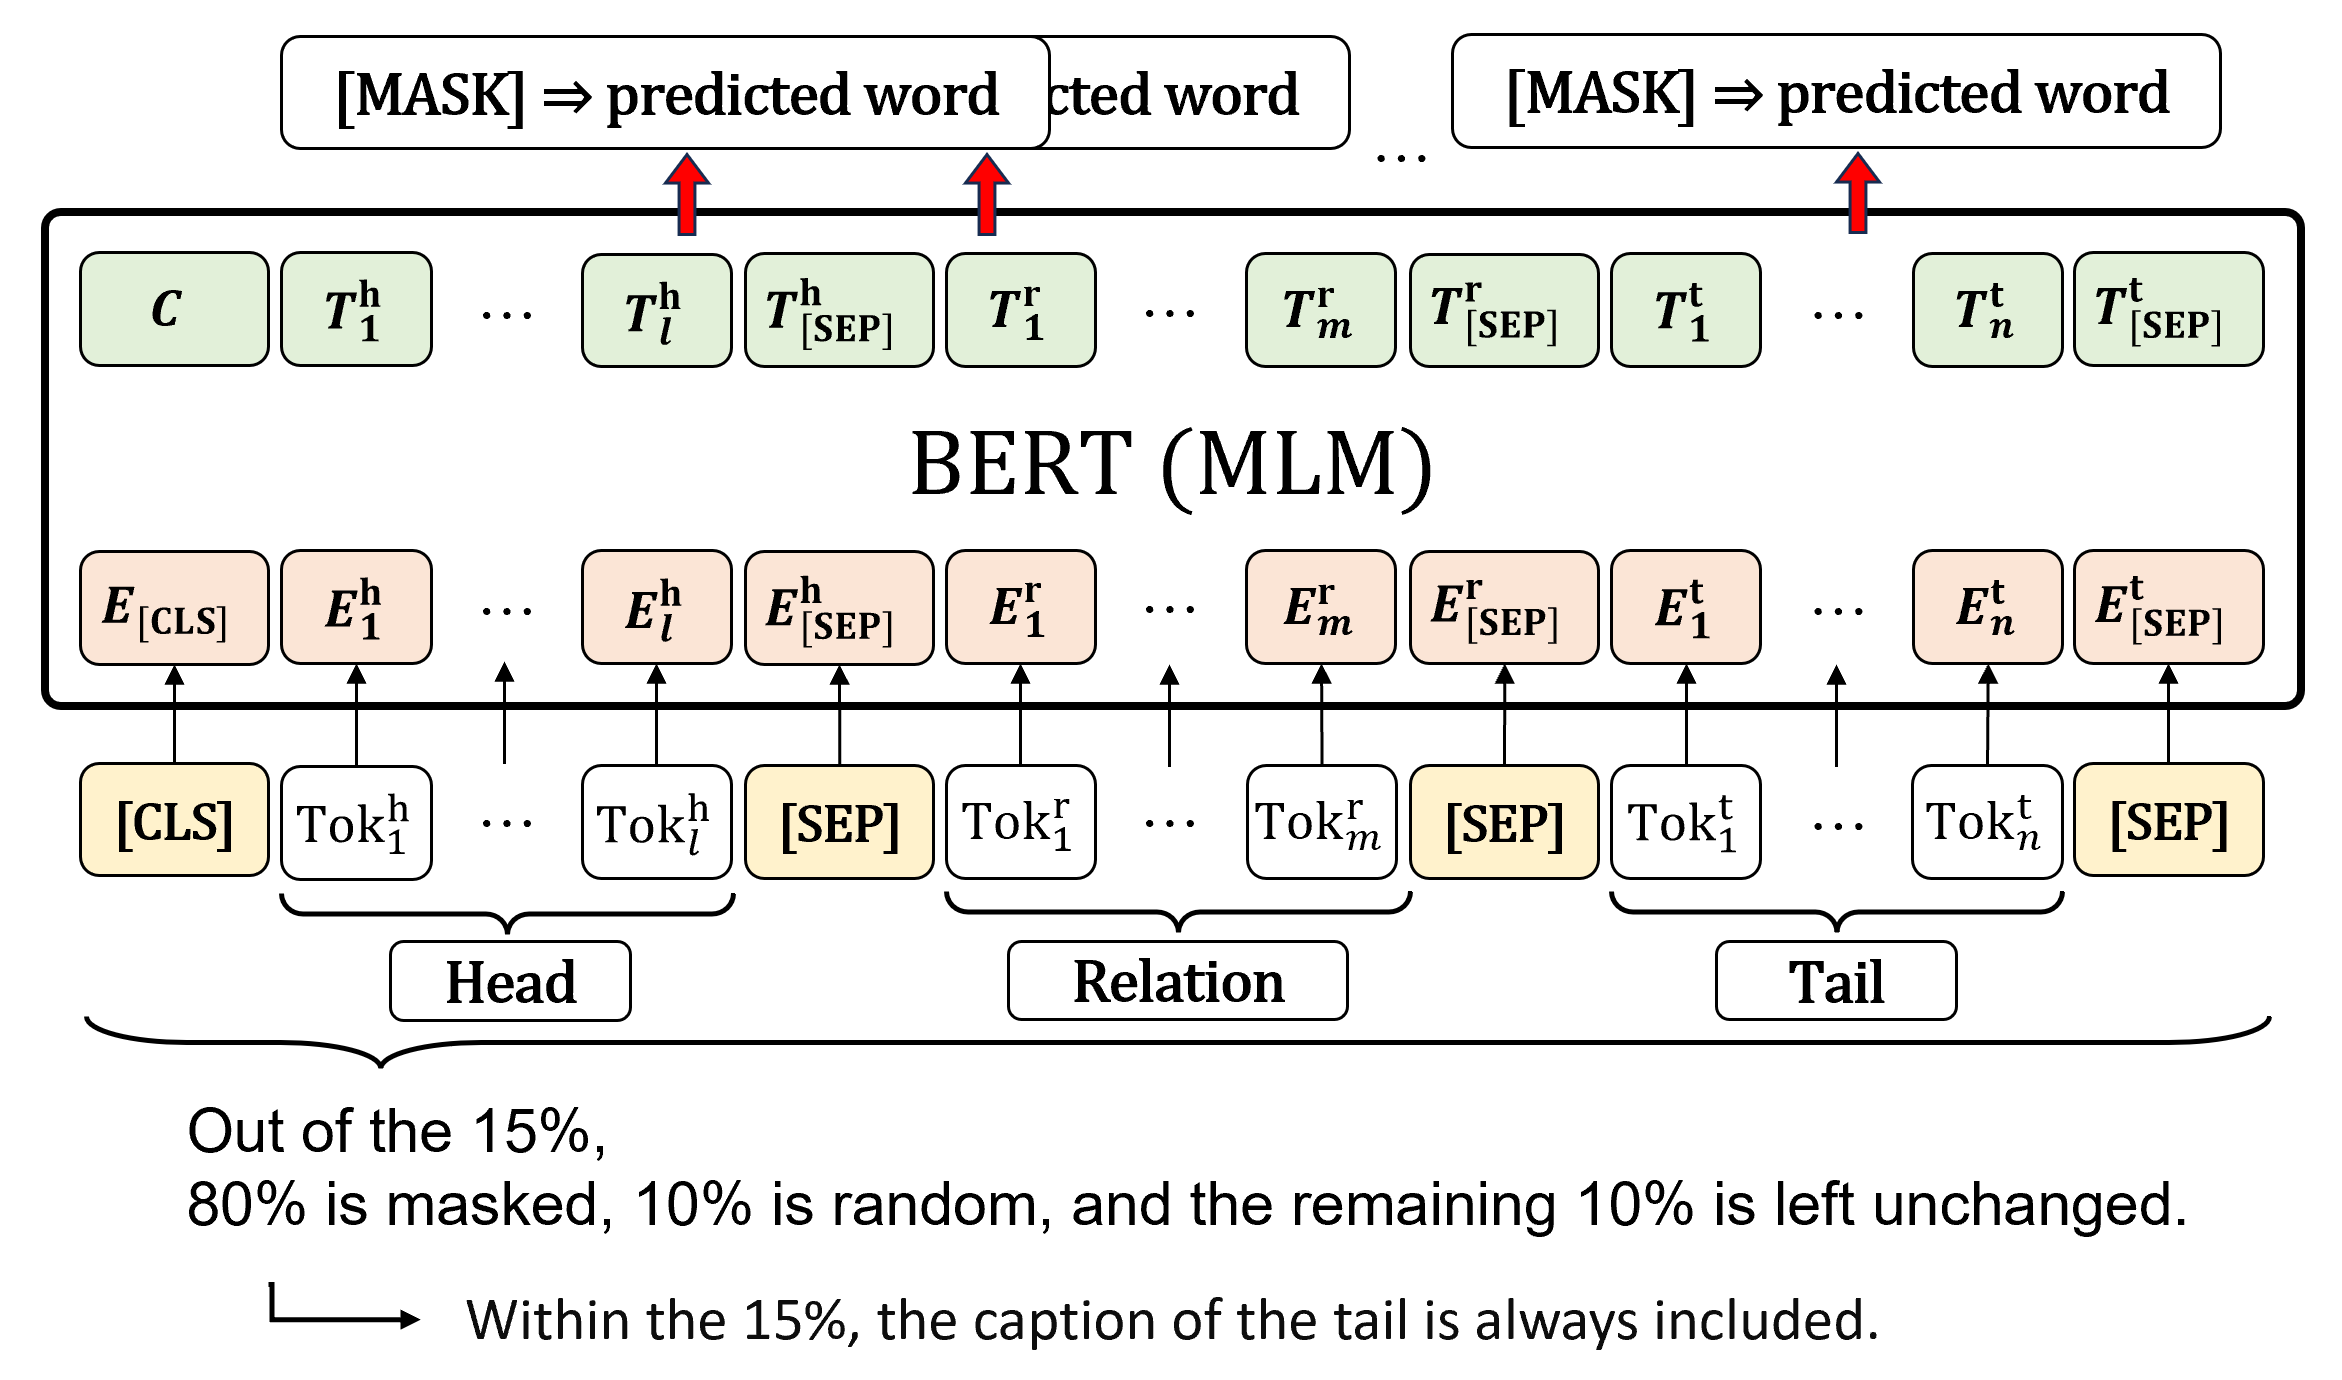
\includegraphics[width=16cm]{assets/MLM_fine-tuning_English.png}
    \caption{BERT の MLM による fine-tuning の概略図}
    \label{MLM_fine_tuning}
\end{figure}
